\chapter{System Design and Architecture}

This chapter describes the design of the proposed digital vault system. The previous chapter introduced the background technologies; this chapter explains how those technologies are combined into a working architecture.

\section{Design Goals}

The main design goal of the project is to provide an encrypted storage vault that can be opened through biometric authorization while still behaving like normal storage after it is unlocked. The system should not require the user to manually run cryptographic commands or remember a separate disk password during daily use. At the same time, the encryption itself should rely on standard and mature Linux storage mechanisms instead of custom cryptographic code.

The design goals can be summarized as follows:

\begin{itemize}
    \item protect vault contents with standard block-level encryption;
    \item use fingerprint verification as the main access-control step;
    \item avoid storing raw biometric data on the host computer;
    \item keep long-term key control on the firmware side;
    \item use short-lived key material on the host only when required for vault operations;
    \item support common vault lifecycle actions such as create, format, unlock, lock, force-lock, and delete;
    \item prevent the application from remaining in an inconsistent state after failed, interrupted, or asynchronous operations;
    \item provide a graphical interface for the major workflows without hiding important security events from the user.
\end{itemize}

These goals shaped the decision to separate the project into hardware, host-control, and storage-management components. Each part has a limited responsibility, which makes the system easier to test and easier to reason about.

\begin{figure}[!htbp]
    \centering
    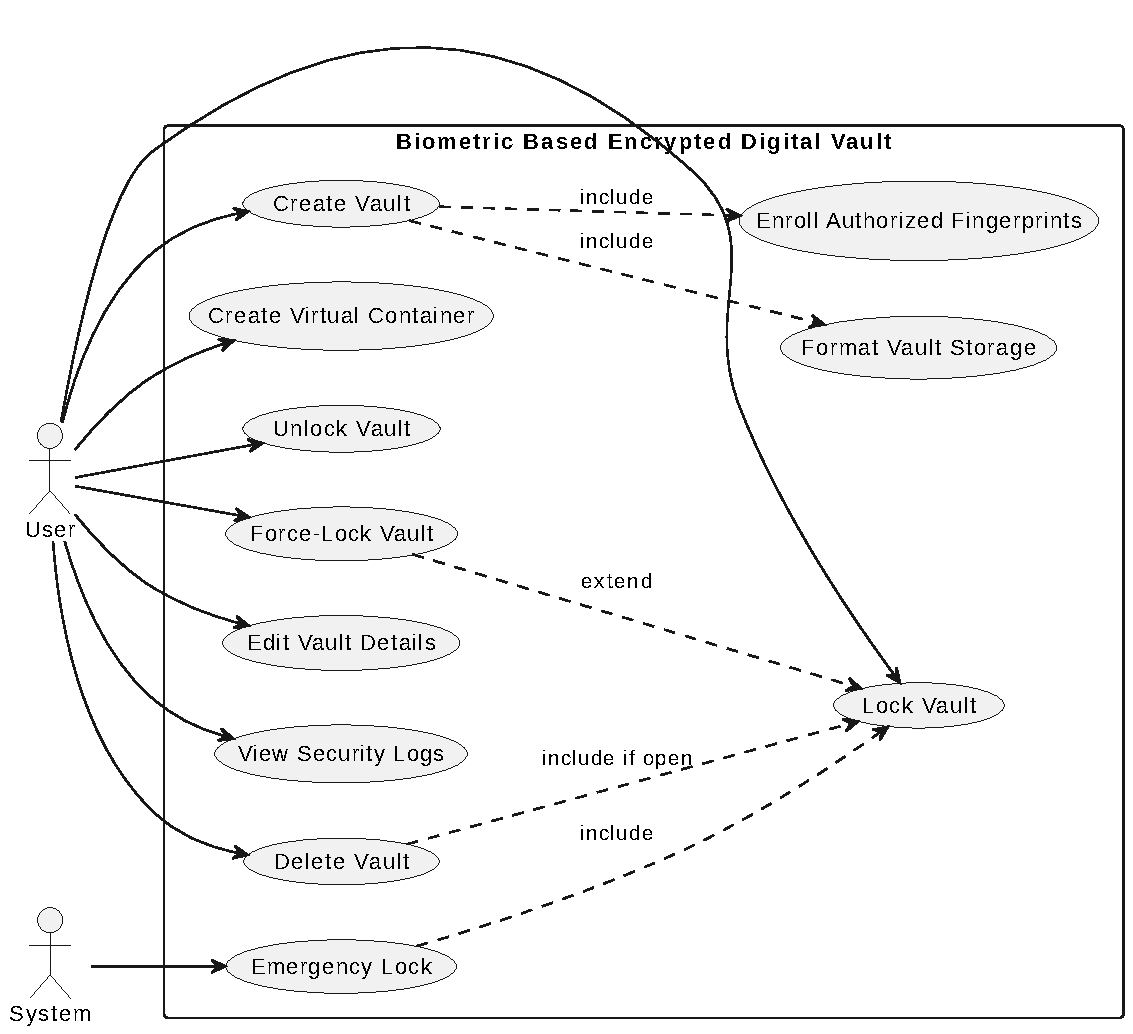
\includegraphics[width=0.98\textwidth,height=0.78\textheight,keepaspectratio]{use_case_diagram.pdf}
    \caption{\label{fig:use-case-diagram}Use-case diagram of the digital vault system.}
\end{figure}

\section{Overall Architecture}

The system is built around three main layers: the biometric hardware layer, the host application layer, and the encrypted storage layer. The biometric hardware layer consists of the AS608 fingerprint sensor, the STM32 Blue Pill microcontroller, and the PL2303 USB-UART bridge. The host application layer contains the Qt/QML graphical interface, the serial/HAL communication logic, and the vault controller. The encrypted storage layer uses LUKS2/dm-crypt and an ext4 filesystem inside the unlocked vault.

\begin{figure}[!htbp]
    \centering
    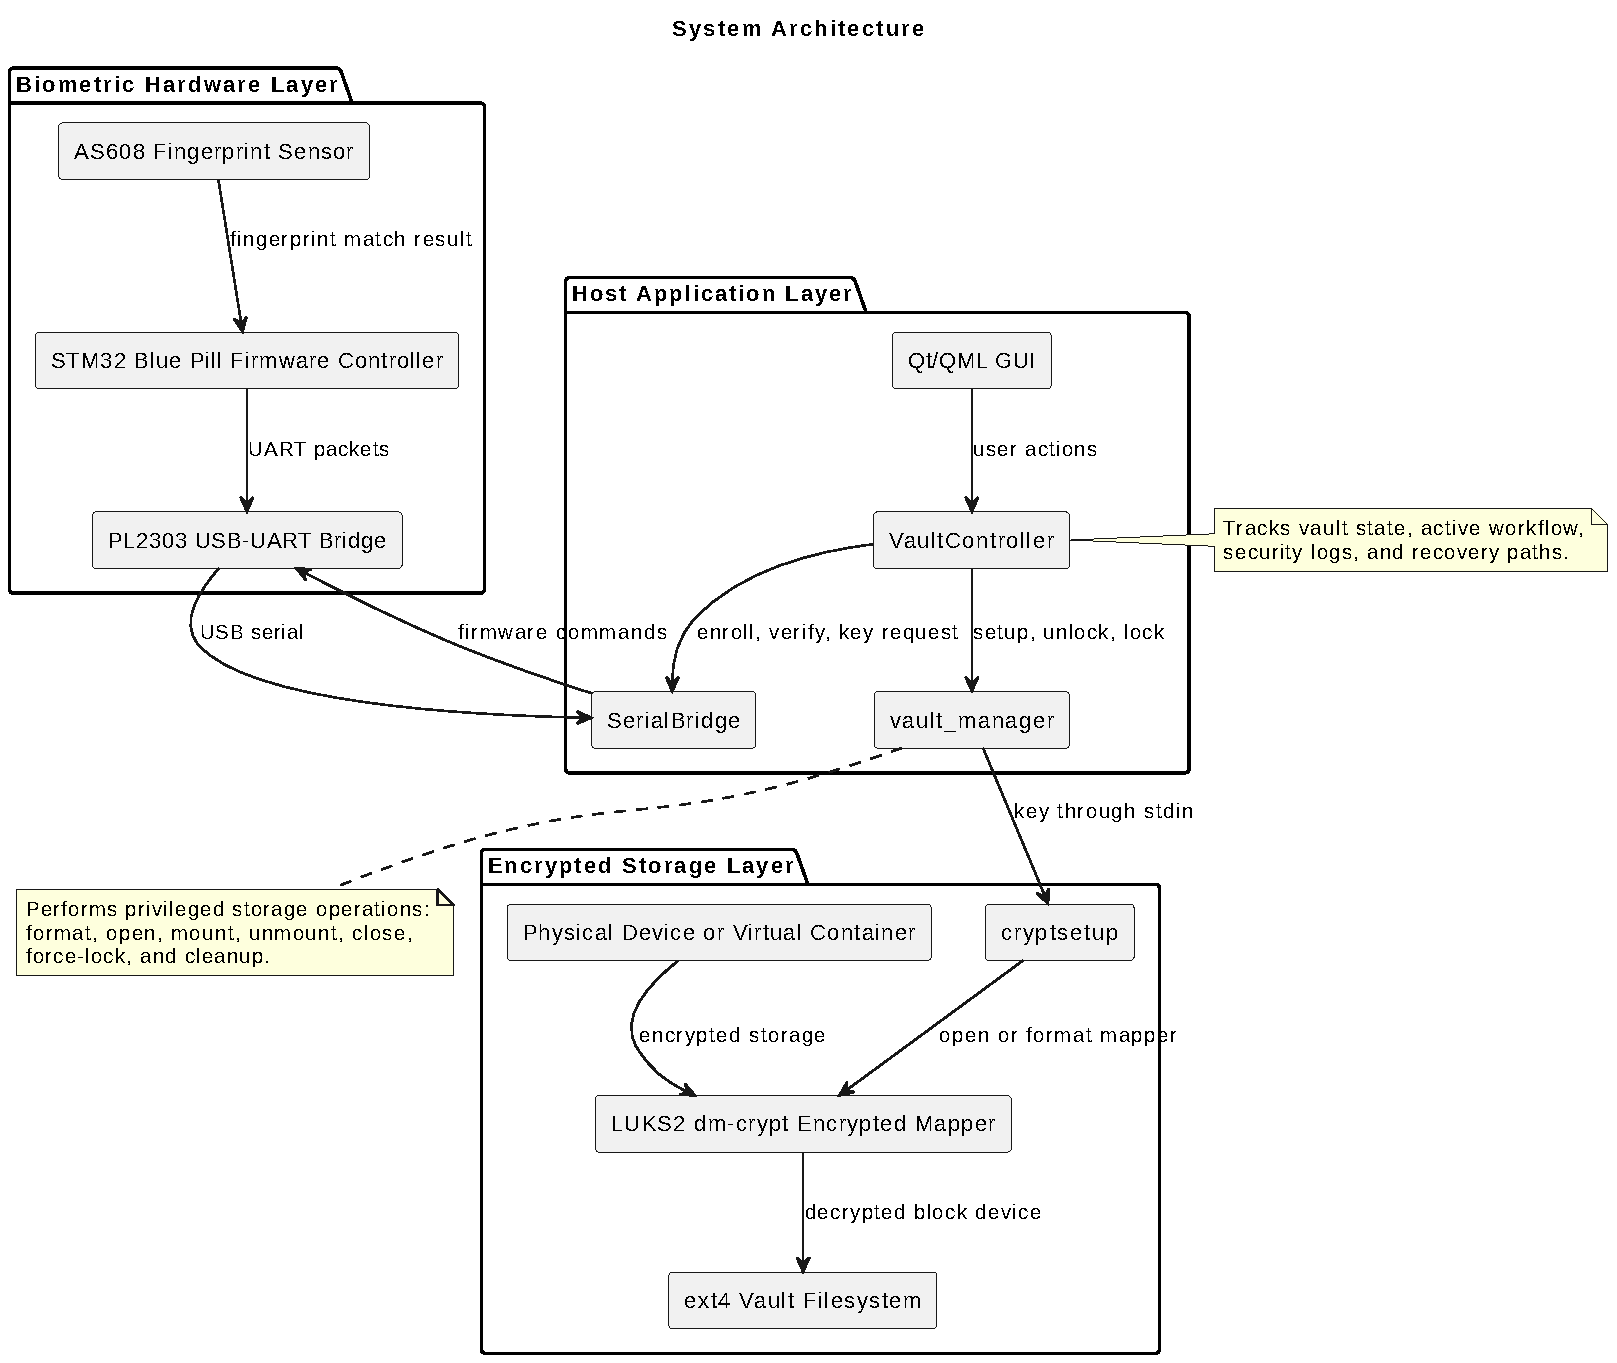
\includegraphics[width=0.98\textwidth,height=0.78\textheight,keepaspectratio]{system_architecture.pdf}
    \caption{\label{fig:system-architecture}System architecture of the digital vault.}
\end{figure}

The host application does not directly implement disk encryption. Instead, it coordinates the user workflow and calls the vault manager for system-level storage operations. The vault manager performs operations such as LUKS formatting, opening the encrypted mapper, mounting the filesystem, unmounting the vault, and closing the mapper. This keeps storage operations in a smaller command-line component while the GUI remains responsible for interaction, status display, and workflow control.

The firmware side is responsible for biometric access decisions and key-release control. The STM32 firmware communicates with the fingerprint sensor and the host, while the host application coordinates the resulting storage workflow. This keeps the overall architecture separated into biometric authorization, host-side workflow control, and encrypted storage management.

\section{Hardware Architecture}

The hardware architecture consists of three main components: the AS608 fingerprint sensor, the STM32 Blue Pill microcontroller, and the PL2303 USB-UART bridge. The AS608 sensor is responsible for biometric enrollment and matching. Fingerprint templates are stored inside the sensor, so the host computer does not need to store raw fingerprint data or template data.

The STM32 Blue Pill works as the controller between the fingerprint sensor and the host computer. It receives commands from the host, drives the fingerprint operation flow, checks sensor results, and sends structured responses back to the host. The firmware also represents the key-control boundary of the system. Vault key material is generated and controlled on the firmware side, and key access is allowed only after a valid fingerprint verification.

The PL2303 USB-UART bridge provides the physical communication path between the STM32 firmware and the computer. From the host side, this appears as a serial port. This choice keeps the hardware connection simple and easy to test while still allowing the project to define its own command and response protocol above the serial link.

The firmware protocol is intentionally small. The host can request operations such as enroll, verify, delete, list enrolled fingerprints, cancel, check status, and request key material after verification. The firmware responds with success, failure, timeout, busy, sensor error, or key-data messages. This small command set is enough for the vault workflows while keeping the firmware interface understandable.

\section{Software Architecture}

The software architecture is divided into the graphical application, the serial communication layer, the vault controller, and the vault manager. This separation was chosen because not every part of the application should have the same responsibility. The vault controller manages the GUI-side workflow, while the vault manager handles storage requests coming from the controller and returns the operation result back to the application.

The Qt/QML graphical interface provides the user-facing workflows. It presents available storage devices, vault status, setup steps, fingerprint prompts, security logs, and vault details. The GUI does not directly format disks or call cryptographic tools. Instead, it calls methods exposed by the vault controller and updates itself based on controller state.

The vault controller is the central coordinator on the GUI side of the host application. It tracks the selected device, current lock state, setup state, fingerprint operation state, auto-lock timer, registered vaults, and security logs. It starts long-running operations asynchronously and updates the GUI through signals and state properties. It also decides which workflow is active, such as vault setup, unlock, delete confirmation, or fingerprint enrollment. The controller does not directly mount disks or format encrypted volumes; it validates the current state and requests the required operation from the vault manager.

The serial communication layer, represented by the serial bridge, handles the STM32 connection. It opens the configured serial port, sends firmware commands, parses firmware responses, emits sensor events, and reports completed operations back to the vault controller. This keeps low-level packet handling away from the GUI and allows the vault controller to work with higher-level events such as ``verification completed'' or ``key received''.

The vault manager is a separate command-line component on the lower-level storage side. It handles system-level storage operations, including LUKS formatting, opening and closing the dm-crypt mapper, mounting and unmounting the ext4 filesystem, creating loop devices, deleting vault partitions, and force-closing busy vault mounts. The GUI does not run these commands directly. For example, during unlock, the controller first completes the fingerprint and key-access workflow, then asks the vault manager to open and mount the encrypted storage. The manager performs the operation and returns success or failure so that the GUI can show the correct state.

\section{User Interface Design Considerations}

The graphical interface was designed with basic human-computer interaction principles in mind. Since the project includes destructive actions such as formatting a storage device or deleting a vault, the interface should help the user understand the current state and avoid accidental actions.

One important principle is recognition over recall. The user should not need to remember device paths, command-line options, mount states, or cryptographic commands. Instead, the interface presents discovered storage devices, registered vaults, lock status, sensor status, and available actions as visible choices. This reduces the mental effort required to operate the vault.

The interface also tries to preserve the user's existing mental model of storage. A user is already familiar with choosing a storage device, opening a folder, copying files, and closing or removing the device when finished. The vault workflow follows this real-world model: after biometric unlock, the vault appears as an accessible folder; after locking, it becomes unavailable again. The encryption and mapper operations remain behind this familiar interaction pattern.

The interface also follows the idea of visibility of system status. States such as locked, unlocked, setup running, sensor disconnected, fingerprint prompt active, or mount busy are shown through the GUI instead of being hidden in terminal output. This helps the user's mental model match the real system state, especially because vault operations can be asynchronous and may take time.

Error prevention was also considered in the workflow design. Formatting, force-formatting, vault deletion, and force-locking are not treated as ordinary one-click actions. The interface uses warnings, previews, confirmation dialogs, and biometric gates where appropriate. These steps are not only usability details; they also reduce the chance of data loss or unintended security changes.

\section{Vault Storage Design}

The vault storage design is based on an encrypted block device. The project can work with a physical block device, such as a USB storage device, or with a virtual container created from a sparse image and attached as a loop device. This gives the user two storage choices: a vault can be created on real removable storage, or a virtual storage file can be created and used as the vault device.

During vault setup, the selected storage target is checked before formatting. If the target already contains a LUKS vault, the setup operation is stopped and the user is informed. If existing data is detected, formatting is also stopped unless the user explicitly chooses a force-format path. Vault creation overwrites the target, so this check is the last line of defense against wiping the wrong device.

The storage target can be used as a full encrypted vault or split into two partitions. In the split mode, the first partition becomes the encrypted vault partition and the second partition becomes a normal storage partition. The normal partition can be formatted with a selected filesystem such as exFAT, FAT32, ext4, NTFS, XFS, or Btrfs. This design allows a device to contain both a protected vault area and a normal visible storage area.

The encrypted vault itself is formatted as a LUKS2 container using AES-256-XTS through dm-crypt. After the container is opened, an ext4 filesystem is created inside the decrypted mapper. The setup flow temporarily mounts the new filesystem to set file ownership for the real user, then unmounts it and closes the mapper. After setup, the vault remains locked until the user performs a biometric unlock.

\begin{table}[H]
\centering
\caption{\label{tab:vault-storage-layout}Vault storage layout options.}
\begin{tabularx}{\textwidth}{lXX}
\toprule
Mode & Storage layout & Use case\\
\midrule
Full-device vault & The selected block device or loop device is formatted as one LUKS2 vault & Simple secure storage device with one protected area\\
Split device & Partition 1 is the encrypted vault; partition 2 is normal storage & Removable storage with both private and ordinary space\\
Virtual container & A sparse image is attached as a loop device and then used like a block device & User-created virtual storage that can also be used as a vault\\
\bottomrule
\end{tabularx}
\end{table}

When the vault is unlocked, the vault manager opens the LUKS2 container as a dm-crypt mapper and mounts the ext4 filesystem at the configured mount point. From the user's perspective, the vault then behaves like a normal folder. When the vault is locked, the filesystem is unmounted and the mapper is closed. This separation keeps encryption below the filesystem layer while still allowing applications and file managers to interact with files normally after unlock.

\section{Authentication and Key Access Flow}

The authentication flow is designed around the idea that fingerprint verification controls access to the vault key. The fingerprint itself is not used as a cryptographic key. Instead, the AS608 sensor performs biometric matching, the STM32 firmware controls the verification flow, and the host requests key access only after successful verification.

There are two main key-access situations: vault setup and vault unlock. During setup, the system needs vault-specific key material to format the new LUKS2 container. LUKS2 stores the required protected keyslot information in its header, not the plaintext key itself. During unlock, the system needs the corresponding vault key material to open the existing LUKS2 container. In both cases, the key material is managed on the firmware side and used by the host only for the minimum time needed to perform the storage operation.

The host-side controller treats fingerprint operations as explicit flows. A verification result is interpreted according to the current state: setup confirmation, unlock, delete confirmation, or another controlled operation. The same physical action, scanning a finger, can mean very different things depending on the active workflow, so the controller has to know which flow it is in before acting on a result.

After key material reaches the host for a setup or unlock operation, it is passed to the vault manager for the required \texttt{cryptsetup} command through standard input instead of command-line arguments. The key buffer is wiped after use, and no persistent host-side copy is kept.

Key access is only needed for operations that open or initialize encrypted storage. Vault setup uses the key to format the new LUKS2 container and create the ext4 filesystem. Vault unlock uses the corresponding vault key to open the existing container and mount the filesystem. Locking does not need the key, because it only unmounts the filesystem and closes the mapper. Vault deletion may still use a biometric gate as a safety step, but the vault key is not needed to remove encrypted data or container metadata.

\begin{figure}[!htbp]
    \centering
    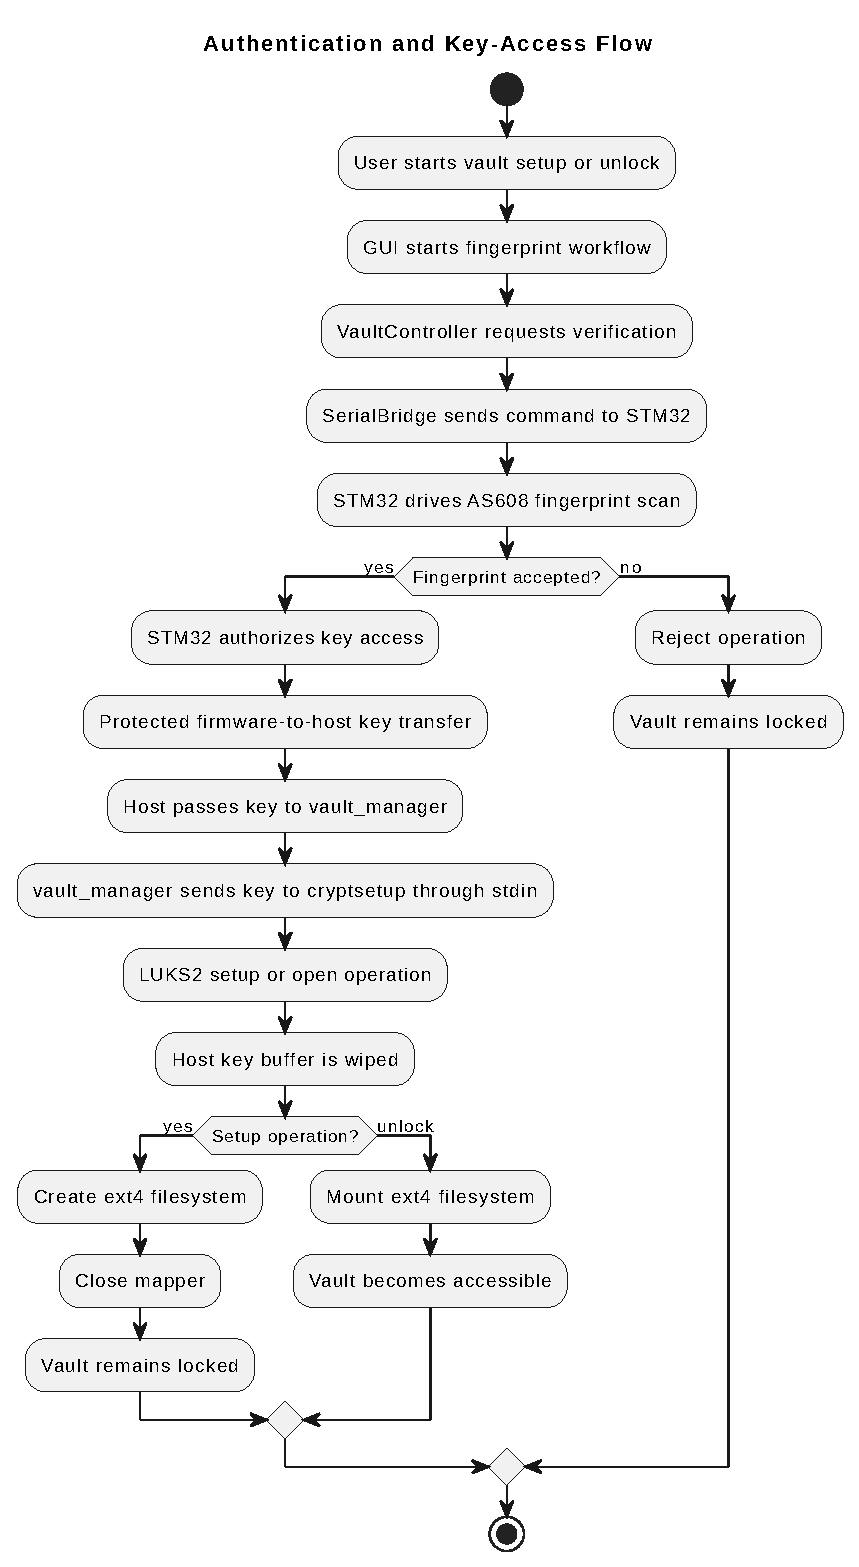
\includegraphics[width=1.00\textwidth,height=0.86\textheight,keepaspectratio]{authentication_key_flow.pdf}
    \caption{\label{fig:auth-key-flow}Authentication and key-access flow.}
\end{figure}

\begin{figure}[!htbp]
    \centering
    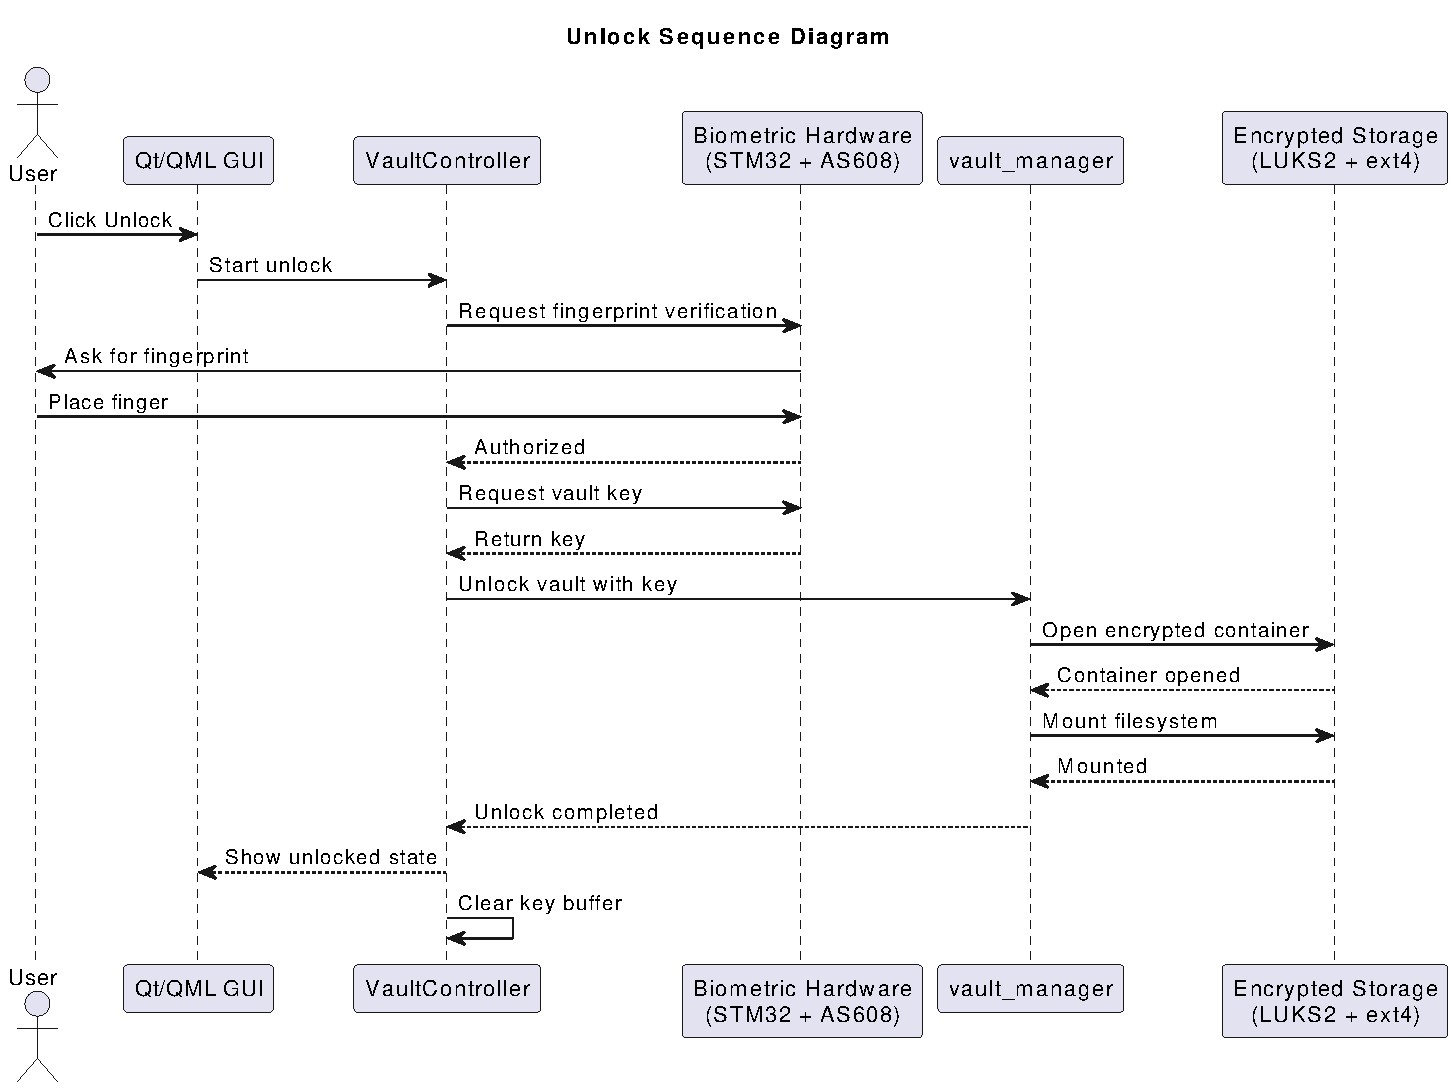
\includegraphics[width=1.00\textwidth,height=0.86\textheight,keepaspectratio]{sequenceunlock.pdf}
    \caption{\label{fig:unlock-sequence}Unlock sequence diagram.}
\end{figure}

\section{Vault Lifecycle}

The vault lifecycle describes how a storage target becomes a protected vault, how it is opened for use, and how it is safely closed or removed. The system is designed so that each lifecycle step has a clear beginning, expected result, and recovery behavior.

\subsection{Vault Creation}

Vault creation starts with selecting a storage target. The target can be a physical block device or a virtual container created by the application. For a virtual container, the application creates a sparse image file, attaches it as a loop device, records the backing image in the vault registry, and then allows the user to continue with the normal vault setup flow.

During setup, the user provides the vault name, storage size options, normal partition options if a split layout is used, and authorized fingerprint information. In the access policy, the fingerprints that can open the vault are defined during vault creation and are not modified later during normal use.

\subsection{Formatting and Initialization}

Formatting is the destructive part of the lifecycle, so the selected device is checked before it is overwritten. If an existing LUKS container or existing data is detected, the setup flow stops unless the user intentionally chooses the force-format path.

After the checks, the vault manager prepares the storage layout. If split mode is selected, it creates a vault partition and a normal partition. The normal partition is formatted with the selected ordinary filesystem. The vault partition is formatted as a LUKS2 container with AES-256-XTS, opened as a dm-crypt mapper, and then formatted as ext4. Finally, the new filesystem is briefly mounted for ownership setup, unmounted, and closed. At the end of initialization, the vault is registered in the application registry and remains locked.

\subsection{Unlock}

Unlocking starts from the graphical interface. The user selects a vault and begins the unlock operation. The controller starts a fingerprint verification flow through the serial bridge and firmware. If the fingerprint is accepted, key access is requested from the firmware side.

The vault manager then uses the key material to open the LUKS2 container and mount the ext4 filesystem. After the vault is mounted, the key material used by the host is wiped. The GUI updates the state to show that the vault is accessible, starts the auto-lock timer, and can open the mount point in the file manager.

\subsection{Lock and Force-Lock}

Normal locking unmounts the vault filesystem and closes the dm-crypt mapper. If no process is using the mount point, this operation is straightforward and the vault returns to the locked state.

If the mount point is busy, the system does not silently ignore the problem. It reports that the vault is in use and can offer a force-lock path. Force-lock first verifies that the mount point belongs to the vault, then stops processes holding the mount, unmounts the filesystem, and closes the mapper. This behavior is useful when a file manager, terminal, or application keeps a file open inside the vault.

\subsection{Auto-Lock and Emergency Lock}

The application supports automatic locking after inactivity. When the vault is open and the configured timeout is reached, the controller starts the lock operation. This reduces the chance of leaving the vault mounted for a long time after the user stops interacting with it.

Emergency locking is used when an unexpected event could leave the system in an unsafe or inconsistent state. Examples include sensor disconnection, application shutdown, startup recovery, or removal of the block device used by the vault. In these cases, the controller tries to reconcile the runtime state and close any remaining mapper or mount that belongs to the vault.

\subsection{Deletion}

Vault deletion is also treated as a controlled lifecycle step. If the vault is open, the system first tries to lock it. For a virtual container, deletion detaches the loop device and removes the backing sparse image. For a physical vault partition, deletion wipes the encrypted vault signature or metadata from the selected partition. The registry is then updated so that the deleted vault is no longer shown as an available managed vault.

\begin{table}[!htbp]
\centering
\caption{\label{tab:vault-lifecycle}Summary of vault lifecycle operations.}
\begin{tabularx}{\textwidth}{lXX}
\toprule
Operation & Main system actions & Expected final state\\
\midrule
Create virtual storage & Create sparse image, attach loop device, register backing file & Virtual storage is available for vault setup\\
Setup vault & Check device, partition if needed, LUKS2 format, ext4 creation, registry update & Vault exists and is locked\\
Unlock vault & Verify fingerprint, access key, open LUKS2 mapper, mount ext4 filesystem & Vault is mounted and accessible\\
Lock vault & Unmount filesystem and close mapper & Vault is locked\\
Force-lock vault & Stop holders if needed, unmount, close mapper, reconcile runtime state & Vault is locked even after busy mount state\\
Auto-lock & Trigger normal lock after inactivity timeout & Vault returns to locked state\\
Emergency lock & Reconcile mapper and mount after disconnection or abnormal state & Runtime state is cleaned up\\
Delete vault & Lock if needed, wipe vault or remove backing image, update registry & Vault is removed from managed devices\\
\bottomrule
\end{tabularx}
\end{table}

\begin{figure}[!htbp]
    \centering
    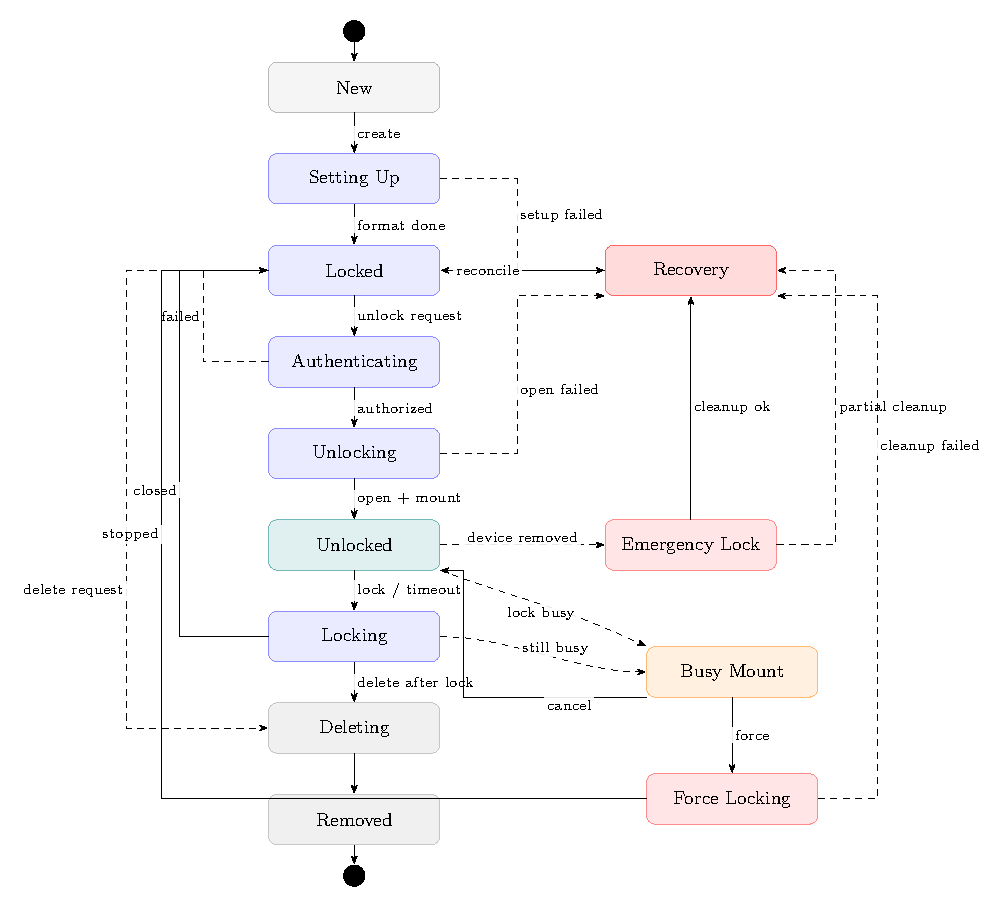
\includegraphics[width=1.00\textwidth,height=0.86\textheight,keepaspectratio]{cycle.pdf}
    \caption{\label{fig:vault-lifecycle-state}Vault lifecycle state diagram.}
\end{figure}

\section{Asynchronous Workflow and State Consistency}

One of the important design challenges in this project is keeping the system out of unstable intermediate states. Vault operations are not simple instant function calls. Formatting a device, opening a LUKS container, mounting a filesystem, waiting for fingerprint input, detecting sensor disconnection, and handling user cancellation are all operations that can take time or fail halfway through. If these operations are handled carelessly, the system can be left in a confusing state, such as a mapper being open without a mount point, a GUI showing the wrong lock status, or a fingerprint enrollment flow continuing after the sensor connection is lost.

For this reason, the host-side design uses asynchronous operations and explicit state tracking. Long-running vault operations are executed outside the main GUI flow so that the interface does not freeze. The controller tracks whether setup, unlock, lock, or fingerprint operations are active, and the UI reacts to these states instead of assuming that every operation succeeds immediately.

The design also treats cleanup as part of the normal workflow, not only as error handling. When a lock operation fails because the mount point is busy, the system reports this state and can offer a force-lock path. When the application starts, it can reconcile leftover runtime state such as an open mapper or stale mount. When the sensor or the block device is disconnected, emergency locking is used to reduce the chance of leaving the vault accessible in an unintended way.

State-machine style thinking is especially important for fingerprint operations. Enrollment, verification, unlock, setup, force-lock confirmation, and delete confirmation flows have different meanings even though they all use the same physical sensor. Treating them as separate states prevents a callback from one flow from accidentally completing another flow. For example, a successful fingerprint scan during vault setup should not be interpreted as a normal unlock unless the controller is actually in the unlock state.

The same idea is used for storage operations. The system distinguishes between a locked vault, an unlocked and mounted vault, an open mapper without a mount, a busy mount point, and a device that has disappeared. These states are not all the same from a security or recovery perspective. By making these states explicit, the application can choose safer recovery behavior instead of relying only on a simple locked/unlocked flag.

\section{Design Alternatives}

Before settling on the current LUKS2/dm-crypt based design, a FUSE-based filesystem approach was considered. The idea was to implement a user-space filesystem where project code would run before file operations. In that design, read operations could trigger decryption, write operations could trigger encryption, and fingerprint verification could be requested when the key was not available.

This approach was attractive because it gave very fine control over file access. The system could decide what to do for each filesystem operation and could theoretically combine authentication, encryption, and file access policy in one place. It also matched the first intuition of the project: every file operation should pass through the biometric vault logic.

However, a filesystem has many more responsibilities than simply reading and writing file contents. It must handle metadata, permissions, renaming, directory traversal, partial writes, random access, file handles, caching behavior, concurrent access, and error cases. In an early experiment, getting large-file reads and concurrent access to behave correctly already took more effort than the rest of the vault logic put together, and that was before any security feature was added on top. Large files also raised performance concerns, since every operation crosses the boundary between the kernel and the user-space filesystem process.

The design therefore moved to block-level encryption with LUKS2/dm-crypt. Encryption now sits below the filesystem layer: the Linux storage stack handles normal filesystem behavior, while the project focuses on vault setup, biometric authentication, key access, GUI workflow, and runtime safety. Put differently, the work shifted away from implementing a custom encrypted filesystem and toward controlling access to a standard encrypted storage volume.

\begin{table}[!htbp]
\centering
\caption{\label{tab:design-alternatives}Comparison of considered storage design alternatives.}
\begin{tabularx}{\textwidth}{lXX}
\toprule
Approach & Advantages & Reasons for not choosing as main design\\
\midrule
FUSE-based encrypted filesystem & Fine-grained control over file operations and authentication points & Complete filesystem behavior is complex; large-file performance and edge cases require careful handling\\
Application-level encrypted container & Simple to keep encryption inside one application & Files are mainly accessible through the application instead of behaving like normal mounted storage\\
LUKS2/dm-crypt encrypted block device & Standard Linux storage encryption, normal filesystem behavior after unlock, mature tooling & Requires careful key handling and mount/unmount cleanup\\
\bottomrule
\end{tabularx}
\end{table}

\section{Security Considerations}

The previous sections described the mechanics of the system. From a security perspective, the main point is the separation of trust boundaries: biometric matching, key-release control, host workflow coordination, and encrypted storage are handled by different parts of the system. This prevents the GUI or storage manager from becoming responsible for every sensitive decision.

Key exposure is intentionally limited. The host receives key material only for operations that require it, such as vault setup or unlock, and does not keep it persistently. The protected firmware-to-host channel and short host-side key lifetime reduce the situations in which key material is exposed.

Biometric data is handled with the same boundary-based approach. Fingerprint verification is treated as an authorization step rather than as a way to derive the encryption key, keeping biometric handling separate from disk encryption.

The access model is designed to be stable after setup. Authorized fingerprints are selected during vault creation, and the normal workflow does not modify the access list later. This makes vault ownership easier to reason about and avoids changing access rights after the vault has already been created.

Runtime protection is still necessary because an unlocked vault behaves like a normal mounted filesystem. Auto-lock and emergency lock reduce the time and situations in which the vault remains mounted unintentionally. Events such as sensor disconnection, abnormal runtime state, or removal of the block device are treated as security-relevant failures, not only as hardware errors.

The main security limitation is that the project protects data at rest and controls the unlock process; it does not make an already compromised host trustworthy. If the host is compromised while the vault is unlocked, mounted files may still be accessible through the operating system. For this reason, the design focuses on controlled unlock, short host-side key lifetime, consistent locking behavior, and encrypted storage when the vault is closed.

\begin{table}[!htbp]
\centering
\caption{\label{tab:threat-mitigation}Threat and mitigation summary.}
\small
\begin{tabularx}{\textwidth}{lXX}
\toprule
Threat or risk & Mitigation in the design & Points to consider\\
\midrule
Lost or stolen storage device & Vault contents are protected with LUKS2/dm-crypt and AES-256-XTS & The protection applies when the vault is locked\\
Wrong or unauthorized fingerprint & The firmware rejects the unlock request if the fingerprint does not match & Access depends on the enrolled fingerprints and the sensor result\\
Biometric template exposure & Fingerprint templates remain inside the AS608 sensor & Physical attacks on the sensor are not handled by the host software\\
Key leakage from host storage & Host does not persistently store the vault key and clears key buffers after use & The host must still be trusted while the key is being used\\
Plaintext key transmission & Firmware-to-host key transfer is protected & The embedded side must also be kept secure\\
Vault left mounted unintentionally & Auto-lock, emergency lock, and shutdown cleanup reduce exposure time & Files are still accessible while the vault is mounted\\
USB storage removal during use & Device removal is treated as abnormal runtime state and triggers recovery behavior & Active file operations can still be interrupted\\
Busy mount during lock & Force-lock path handles processes that keep files open & The user may need to confirm closing active processes\\
\bottomrule
\end{tabularx}
\end{table}

In summary, the design does not rely on a single protection point. Biometric matching limits who can request access, firmware-side key control limits where long-term key authority is placed, protected transfer and short host-side key lifetime reduce key exposure during unlock, and LUKS2/dm-crypt protects the stored data while the vault is closed. Runtime mechanisms such as auto-lock, emergency lock, and recovery handling cover the period after the vault has been opened, when ordinary applications can access the mounted filesystem.
